\begin{figure}[h]
    \centering

\tikzset{every picture/.style={line width=0.75pt}} %set default line width to 0.75pt        

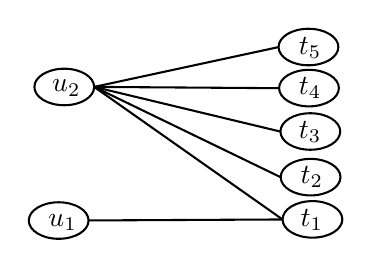
\begin{tikzpicture}[x=0.75pt,y=0.75pt,yscale=-.55,xscale=.9]
%uncomment if require: \path (0,310); %set diagram left start at 0, and has height of 310

%Shape: Circle [id:dp7530951281094582] 
\draw   (257.14,91.73) .. controls (257.17,100.56) and (250.04,107.76) .. (241.2,107.79) .. controls (232.37,107.83) and (225.17,100.7) .. (225.14,91.86) .. controls (225.1,83.02) and (232.23,75.83) .. (241.07,75.79) .. controls (249.91,75.76) and (257.1,82.89) .. (257.14,91.73) -- cycle ;
%Shape: Circle [id:dp9324922852398969] 
\draw   (256.86,55.73) .. controls (256.9,64.56) and (249.76,71.76) .. (240.93,71.79) .. controls (232.09,71.83) and (224.9,64.7) .. (224.86,55.86) .. controls (224.82,47.03) and (231.96,39.83) .. (240.79,39.8) .. controls (249.63,39.76) and (256.82,46.89) .. (256.86,55.73) -- cycle ;
%Shape: Circle [id:dp21183658776860814] 
\draw   (126.14,90.73) .. controls (126.17,99.56) and (119.04,106.76) .. (110.2,106.79) .. controls (101.37,106.83) and (94.17,99.7) .. (94.14,90.86) .. controls (94.1,82.02) and (101.23,74.83) .. (110.07,74.79) .. controls (118.91,74.76) and (126.1,81.89) .. (126.14,90.73) -- cycle ;
%Shape: Circle [id:dp1138329234262836] 
\draw   (257.86,129.73) .. controls (257.9,138.56) and (250.76,145.76) .. (241.93,145.79) .. controls (233.09,145.83) and (225.9,138.7) .. (225.86,129.86) .. controls (225.82,121.03) and (232.96,113.83) .. (241.79,113.8) .. controls (250.63,113.76) and (257.82,120.89) .. (257.86,129.73) -- cycle ;
%Shape: Circle [id:dp5258577677891723] 
\draw   (123.14,207.73) .. controls (123.17,216.56) and (116.04,223.76) .. (107.2,223.79) .. controls (98.37,223.83) and (91.17,216.7) .. (91.14,207.86) .. controls (91.1,199.02) and (98.23,191.83) .. (107.07,191.79) .. controls (115.91,191.76) and (123.1,198.89) .. (123.14,207.73) -- cycle ;
%Shape: Circle [id:dp23423166586948985] 
\draw   (258,169.73) .. controls (258.03,178.56) and (250.9,185.76) .. (242.06,185.79) .. controls (233.23,185.83) and (226.03,178.7) .. (226,169.86) .. controls (225.96,161.03) and (233.09,153.83) .. (241.93,153.79) .. controls (250.76,153.76) and (257.96,160.89) .. (258,169.73) -- cycle ;
%Shape: Circle [id:dp9473655596063126] 
\draw   (259,206.73) .. controls (259.03,215.56) and (251.9,222.76) .. (243.06,222.79) .. controls (234.23,222.83) and (227.03,215.7) .. (227,206.86) .. controls (226.96,198.03) and (234.09,190.83) .. (242.93,190.79) .. controls (251.76,190.76) and (258.96,197.89) .. (259,206.73) -- cycle ;
%Straight Lines [id:da9982536095158081] 
\draw    (123.14,207.73) -- (227,206.86) ;
%Straight Lines [id:da47969048910504686] 
\draw    (126.14,90.73) -- (226,169.86) ;
%Straight Lines [id:da04357275217194001] 
\draw    (126.14,90.73) -- (225.86,129.86) ;
%Straight Lines [id:da5426269746436285] 
\draw    (126.14,90.73) -- (225.14,91.86) ;
%Straight Lines [id:da23827025163526505] 
\draw    (126.14,90.73) -- (224.86,55.86) ;
%Straight Lines [id:da8587083135549514] 
\draw    (126.14,90.73) -- (227,206.86) ;


% Text Node
\draw (234,80) node [anchor=north west][inner sep=0.75pt]   [align=left] {{$t_4$}};
% Text Node
\draw (234,45) node [anchor=north west][inner sep=0.75pt]   [align=left] {{$t_5$}};
% Text Node
\draw (102,82) node [anchor=north west][inner sep=0.75pt]   [align=left] {{$u_2$}};
% Text Node
\draw (100,200) node [anchor=north west][inner sep=0.75pt]   [align=left] {{$u_1$}};
% Text Node
\draw (234,118) node [anchor=north west][inner sep=0.75pt]   [align=left] {{$t_3$}};
% Text Node
\draw (235,158) node [anchor=north west][inner sep=0.75pt]   [align=left] {{$t_2$}};
% Text Node
\draw (235,195) node [anchor=north west][inner sep=0.75pt]   [align=left] {{$t_1$}};
\end{tikzpicture}
\caption{The described instance $\inst$ with $\prob=1/2$ and $\sigmabf = (t_1, \ldots, t_5)$.}\label{fig:instance_generalized_imbalance}
\end{figure}